\documentclass[12pt]{article}
\usepackage{amsmath}
\usepackage[lmargin = 1in, rmargin = 0.8in, tmargin = 1in, bmargin = 1in]{geometry}
\usepackage[none]{hyphenat}
\usepackage{graphicx}
\usepackage{subcaption}
\usepackage{float}
\usepackage{longtable}

\title{\textbf{DESIGN OPTIMIZATION OF BRAKE DISC GEOMETRY}}
\author{\\by \\Abhijeet Durgude\\ Aditya Vipradas\\ Sharan Kishore\\ Swapnil Nimse\\\\\\\\MAE 598-2016-11\\Final Report}
\begin{document}
\maketitle
\vspace{1cm}
\begin{center}
\textbf{ABSTRACT}
\end{center}
The motivation of this project is to determine the optimum dimensions of the brake disc for a four-wheeler vehicle using MATLAB and ANSYS. These dimensions include the disc inner radius, outer radius and thickness. Structural, modal and thermal load cases for emergency braking conditions are individually considered to determine these dimensions. The optimization objective is to minimize the brake disc volume, whereas the other objectives are to minimize the stress, temperature and maximize the first natural frequency of the disc. These goals are accomplished using optimization algorithms in MATLAB and the results are correlated with the values obtained from ANSYS. Finally, system optimization is performed using MOGA by integrating all the load cases. 
\newpage  
\begin{center}
\textbf{ACKNOWLEDGMENTS}
\end{center}
We primarily thank Prof. Yi (Max) Ren for his unconditional support to this project. Moreover, this work would not have been possible without the assistance and resources of the Arizona State University laboratories. Finally, we thank our friends and peers for helping us when required. We also thank our parents for their emotional support.
\newpage
\tableofcontents
\newpage  
\listoffigures
\newpage  
\listoftables
\newpage
\section{Design Problem Statement}
\textbf{Primary objective:} To minimize the brake disc volume for emergency braking conditions\\\\
\textbf{Secondary objectives: }
\begin{itemize}
\item Minimize the maximum stress in the brake disc
\item Maximize the first natural frequency of the brake disc
\item Minimize the maximum temperature in the brake disc
\end{itemize}
\subsection{\textbf{Subsystem 1:} Structural Analysis}
\textbf{Team Member:} Swapnil Nimse 
\newline\newline
The brake disc has to sustain the pressure from the hydraulically actuated brake pads during sudden braking conditions. Stresses are induced due to friction between the brake pads and the disc. The disc also experiences centrifugal body forces due to its rotation. Resultant stresses generated due these forces can lead to material failure. Therefore, it is of prime importance to make sure that the stresses in the disc are minimized. 
\subsection{\textbf{Subsystem 2:} Modal Analysis}
\textbf{Team Member:} Abhijeet Durgude
\newline\newline
Free modal analysis is performed to ensure that the disc's first natural frequency is higher than the engine firing frequency. This guarantees that the disc does not experience failure due to resonance.  
\subsection{\textbf{Subsystem 3:} Thermal Analysis}
\textbf{Team Member:} Sharan Kishore
\newline\newline
Braking in a vehicle takes place due to friction between the brake pads and the rotor disc. This leads to heat flux generation in the disc which consequently results in increase in its temperature and thermal stresses. Emergency braking conditions induce high temperatures that damage the contact surfaces. It is therefore essential to minimize the temperature to prevent disc wear and tear.
\subsection{\textbf{Subsystem 4:} MATLAB Programming}
\textbf{Team Member:} Aditya Vipradas
\newline\newline
Subsystem and system level optimization are performed by programming the entire procedure in MATLAB. This includes the use of optimization algorithms like \emph{interior-point method (fmincon), and Multi-Objective Genetic Algorithm (MOGA)}, plotting the Pareto curves for subsystem and system level optimization and generating results for validation purposes.\newline\newline
The design optimization methodology flowchart is as shown in Figure \ref{fig1}. 
\begin{figure}[H]
\begin{center}
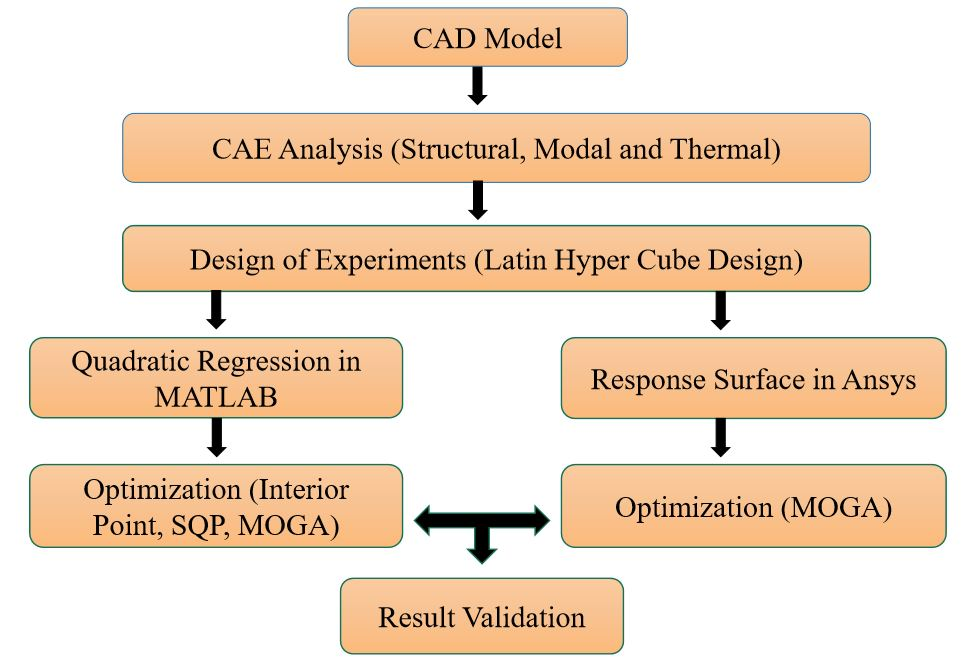
\includegraphics[width=0.9\textwidth]{flow.jpg}
\caption{Design optimization process flowchart}
\label{fig1}
\end{center}
\end{figure}
\section{Nomenclature}
\begin{description}
\item[$V$:] Volume (\textit{$mm^{3}$})
\item[$\alpha$:] Regression coefficients for volume
\item[$S$:]  Stress (\textit{MPa})
\item[$\beta$:] Regression coefficients for stress
\item[$F$:] First natural frequency (\textit{Hz})
\item[$\gamma$:] Regression coefficients for frequency
\item[$T$:] Temperature (\textit{$^{o}C$})
\item[$\delta$:] Regression coefficients for temperature
\item[$P1$:] Inner disc radius (\textit{mm})
\item[$P2$:] Outer disc radius (\textit{mm})
\item[$P3$:] Disc thickness (\textit{mm})
\item[$d$:] Braking distance (\textit{m})
\item[$t_{e}$:] Braking time (\textit{s})
\item[$u$:] Initial vehicle velocity (\textit{kmph})
\item[$m$:] Vehicle mass (\textit{kg})
\item[$\nu$:] Coefficient of friction
\item[$w$:] Disc rotational velocity (\textit{rad/s})
\item[$R_{avg}$:] Average of P1 and P2 (\textit{mm})
\item[$KE$:] Vehicle kinetic energy (\textit{J})
\item[$F_b$:] Total braking force on the disc (\textit{N})
\item[$P$:] Pressure acting on the disc due to one brake pad (\textit{Pa})
\item[$A_{p}$:] Brake pad area (\textit{$mm^{2}$})
\item[$A_{sp}$:] Brake pad swept area (\textit{$mm^{2}$})
\item[$q$:] Heat flux (\textit{$W/m^{2}$})
\item[$T_{amb}$:] Ambient temperature (\textit{$^{o}C$})
\end{description}
\section{Mathematical Model}
The brake disc inner radius (P1), outer radius (P2) and thickness (P3) are the design variables in this optimization study. Initially, structural, modal and thermal analyses are performed in ANSYS. For the assumed geometric constraints, Design Of Experiment (DOE) points are generated. Mathematical model is then generated by performing a $2^{nd}$ order regression analysis on these DOE points to obtain the volume, stress, frequency and temperature quadratic functions. The optimization problem is designed as follows:
\newline\newline
\textbf{Primary objective:} 
\begin{equation}
Minimize: f1: V = \sum_{n=1}^{n=3} \alpha_{n}x_{n} + \sum_{n=4}^{n=6} \alpha_{n}x_{n}^{2} + \alpha_{7} ; (R_{volume}^{2} = 0.98)
\end{equation}
\textbf{Secondary objectives:} 
\begin{equation}
f2: Minimize: S = \sum_{n=1}^{n=3} \beta_{n}x_{n} + \sum_{n=4}^{n=6} \beta_{n}x_{n}^{2} + \beta_{7} ; (R_{stress}^{2} = 0.53) \footnote{$5^{th}$ order polynomial fit gives a better $R^{2}$ value of 0.77. Kriging model may work better as well.}
\end{equation}
\begin{equation}
f3: Maximize: F = \sum_{n=1}^{n=3} \gamma_{n}x_{n} + \sum_{n=4}^{n=6} \gamma_{n}x_{n}^{2} + \gamma_{7} ; (R_{frequency}^{2} = 0.92)
\end{equation}
\begin{equation}
f4: Minimize: T = \sum_{n=1}^{n=3} \delta_{n}x_{n} + \sum_{n=4}^{n=6} \delta_{n}x_{n}^{2} + \delta_{7} ; (R_{thermal}^{2} = 0.97)
\end{equation}
\textbf{Geometrical constraints for all subsystems:} \newline
\begin{equation}
g1: -P1 \le -66
\end{equation}
\begin{equation}
g2: P1 \le 90
\end{equation}
\begin{equation}
g3: -P2 \le -124
\end{equation}
\begin{equation}
g4: P2 \le 150
\end{equation}
\begin{equation}
g5: -P3 \le -5
\end{equation}
\begin{equation}
g6: P3 \le 27
\end{equation}
This is a multi-objective optimization problem. A multi-objective optimization algorithm can be readily solved using MOGA. But MOGA will not always give the best optimum value. Therefore, it is beneficial to convert the multi-objective problem into a single objective problem by assuming the rest of the objectives as constraints. In order to use single-objective optimization algorithms for this problem, it is thus necessary to provide upper or lower bounds on the secondary objective functions. This aids in plotting the desired Pareto curves. The bounds are determined by taking into consideration the brake disc failure.\newline\newline
\textbf{Design constraints:} 
\begin{equation}
g7: S \le 14 MPa
\label{7}
\end{equation}
\begin{equation}
g8: -F \le -1200 Hz
\label{8}
\end{equation}
\begin{equation}
g9: T \le 400^{o}C
\label{9}
\end{equation}
The sub-system level optimization problems are designed as follows:
\subsection{Structural Analysis Model}
$Min: f1, f2$\\\\
s.t.\\  $g1, g2, g3, g4, g5, g6$ and $g7$
\subsection{Modal Analysis Model}
$Min: f1, -f3$\\\\
s.t.\\  $g1, g2, g3, g4, g5, g6$ and $g8$
\subsection{Thermal Analysis Model}
$Min: f1, f4$\\\\
s.t.\\  $g1, g2, g3, g4, g5, g6$ and $g9$

\section{Model Analysis}
The flowchart for optimization in ANSYS is shown in Figure \ref{flow2}. This figure pertains to the flowchart for structural analysis. Similar procedure is followed for modal and thermal analyses.
\begin{figure}[H]
\begin{center}
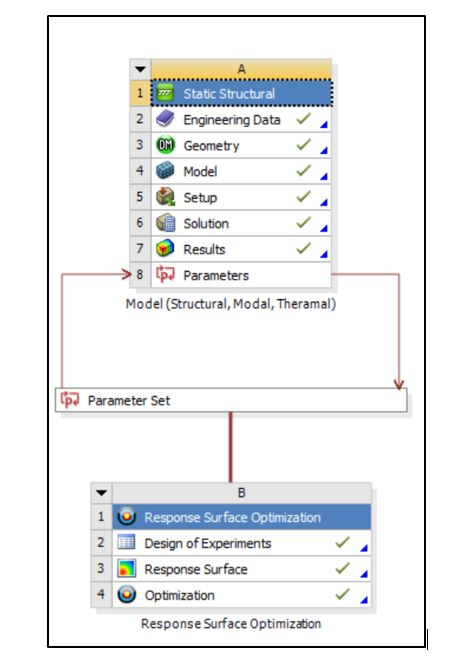
\includegraphics[width=0.5\textwidth]{flow_ansys.jpg}
\caption{ANSYS Optimization Flowchart}
\label{flow2}
\end{center}
\end{figure}
\subsection{FE Model}
The brake disc geometry is prepared in ANSYS DesignModeler as shown in Figure \ref{cad}. The initial values for P1, P2 and P3 are considered to be 75 mm, 125 mm and 25 mm respectively. These values are obtained from the literature survey by considering disc dimensions in different vehicles.
\begin{figure}[H]
\begin{center}
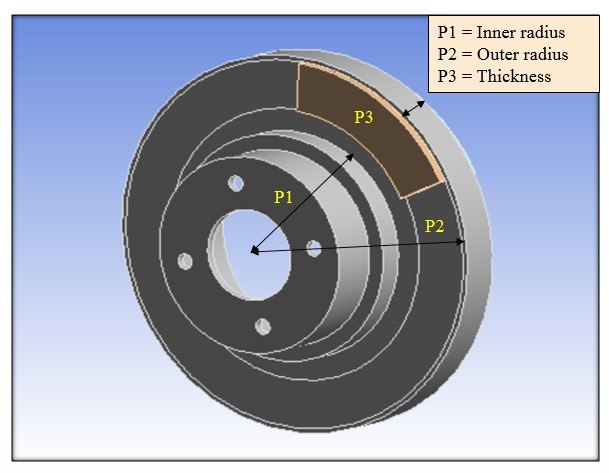
\includegraphics[width=0.55\textwidth]{cad.jpg}
\caption{Disc Brake CAD Model}
\label{cad}
\end{center}
\end{figure}
The CAD geometry is meshed using 6 mm sized tetrahedral quadratic elements as shown in Figure \ref{mesh}.
\begin{figure}[H]
\begin{center}
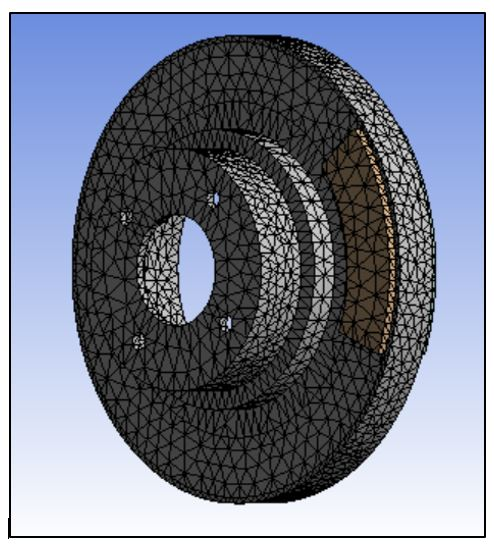
\includegraphics[width=0.4\textwidth]{mesh.jpg}
\caption{Disc Brake Mesh Model}
\label{mesh}
\end{center}
\end{figure}
The brake disc is made of gray cast iron. The material properties of gray cast iron are shown in Table \ref{mat}.
\begin{longtable}{|l|c|c|}
\hline 
\textbf{Property} & \textbf{Value} & \textbf{Unit}\\
\hline
Density & 7200 & $kg/m^{3}$ \\
\hline
Young's modulus & 110 & GPa \\
\hline
Poisson's ratio & 0.28 & -\\
\hline
Thermal conductivity & 52 & $W/m^{o}C$ \\
\hline
Specific heat & 447 & $J/kg^{o}C$  \\
\hline
\caption{Gray cast iron material properties}
\label{mat}
\end{longtable}

The assumptions made for performing the FEM analysis are as follows:
\begin{itemize}
\item The braking torque distribution between the front and rear axles is 70:30.
\item Natural convection takes place due to the ambient air.
\item The disc brake considered is of the solid type.
\item Heat flux on the disc brake acts on both sides of the disc.
\end{itemize}

\subsection{Structural Analysis}
Considering the emergency braking distance of 10 m with stopping time of 5 seconds for a vehicle with initial velocity of 90 km/hr, the braking pressure required is calculated. This pressure will act as one of the boundary conditions for the simulation. It is assumed that 70\% of the braking power is in the front axle of a four-wheeler vehicle. The force acting on a single disc brake is calculated by multiplying the front axle braking power by 0.5. Using this, the pressure on each pad is calculated by considering the coefficient of friction. Here, $d = 10 m; t_{e} = 5 s; u = 90 kmph; m = 1500 kg; \nu = 0.22; A_{p} = 3552 mm^{2}$.\\\\
Calculating the disc angular velocity ($\omega$),
\begin{equation}
\omega = u/R_{avg} = 250 rad/s
\end{equation}
Evaluating the total braking force on the disc ($F_{b}$),
\begin{equation}
F_{b} = (KE*0.5*0.7)/d = 16.406 kN
\end{equation}
Formulating the pressure exerted by one brake pad on the disc ($P$),
\begin{equation}
P = F_{b}/(2*A_{p}*\nu) = 10.495 MPa
\end{equation}
Static structural analysis is performed on the aforementioned geometry due to the brake pad actuating load acting on the disc. The boundary conditions imposed on the brake geometry are as follows. See Figure \ref{bc}.
\begin{itemize}
\item The inner circumference of the wheel hub has a revolute joint applied.
\item The brake caliper pads are constrained in X and Z directions. They are kept free to move in the Y direction.
\item The rotational velocity of 250 rad/s is applied on the disc at the wheel hub attachment point.
\item Frictional contact is provided between the brake caliper pads and brake rotor.
\item Actuating pressure of 10.496 MPa is applied on the brake pads.
\end{itemize}
\begin{figure}[H]
\begin{center}
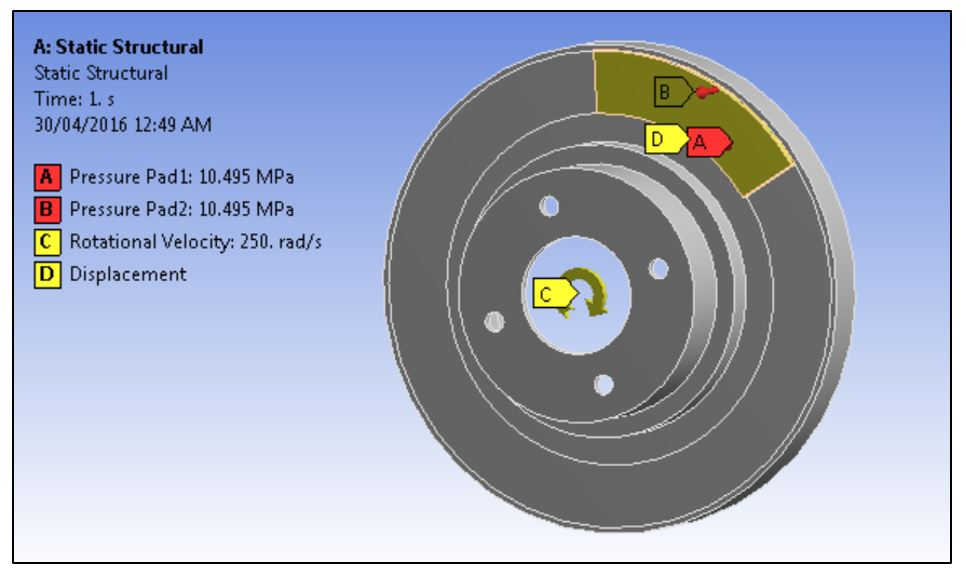
\includegraphics[width=0.6\textwidth]{bc.jpg}
\caption{Static structural boundary conditions}
\label{bc}
\end{center}
\end{figure}
The stress plot obtained is as shown in Figure \ref{stress}. As observed, the maximum stress of 14.262 MPa is obtained for initial conditions on the design variables.
\begin{figure}[H]
\begin{center}
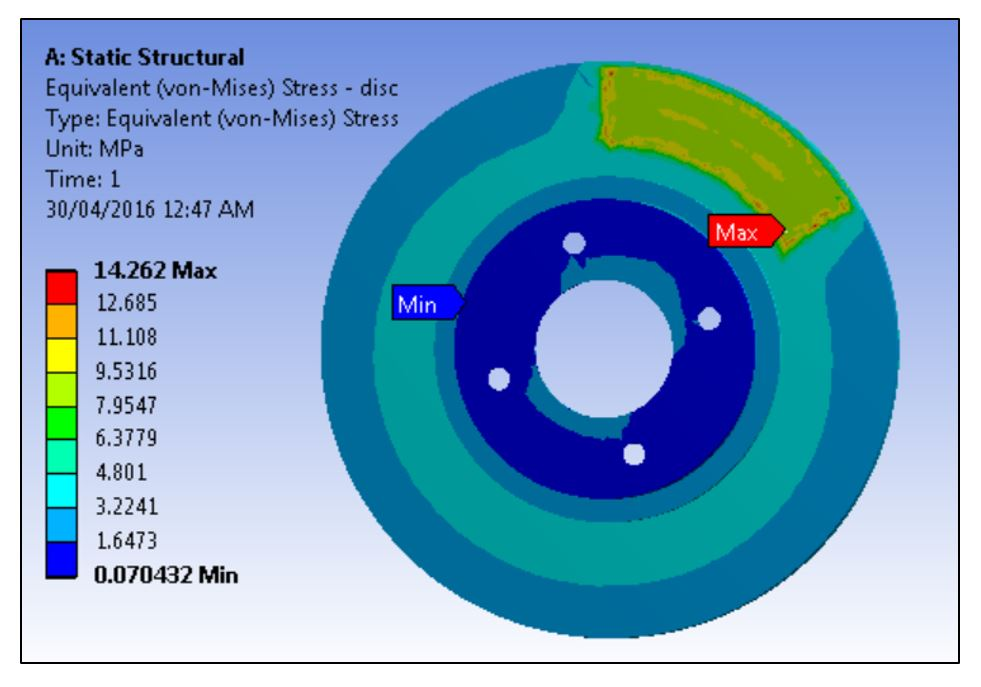
\includegraphics[width=0.6\textwidth]{stress.jpg}
\caption{Stress plot for initial conditions on the design variables}
\label{stress}
\end{center}
\end{figure}

\subsection{Modal Analysis}
Modal analysis is performed on the brake disc to determine its free natural frequency. The brake caliper pad geometry is suppressed while performing this analysis because the natural frequency of the brake disc is to be determined. Figure \ref{mode} shows the first natural frequency and its mode shape.
\begin{figure}[H]
\begin{center}
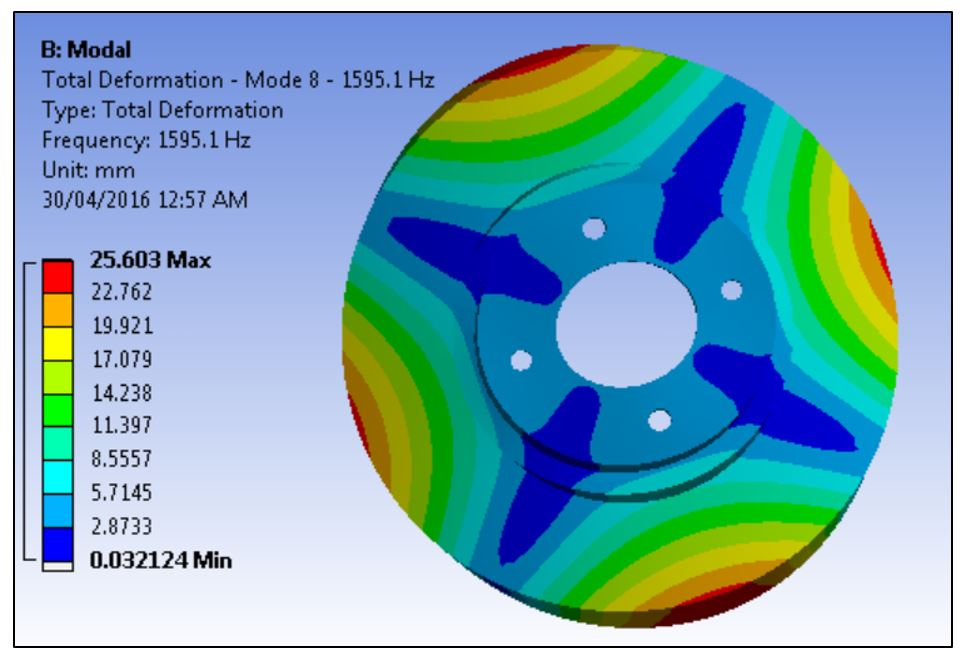
\includegraphics[width=0.6\textwidth]{mode.jpg}
\caption{Mode shape plot for initial conditions on the design variables}
\label{mode}
\end{center}
\end{figure}

\subsection{Thermal Analysis}
Transient thermal analysis is performed on the disc to observe the maximum temperature rise after the braking operation. The heat flux is calculated as shown below. It is assumed that 70\% of the braking power is in the front axle of a four-wheeler vehicle. The total heat flux is also multiplied by 0.5 to get the flux generated by a single pad on the disc brake. Here, $t_{e} = 5 s; A_{sp} = 0.021 m^{2}; T_{amb} = 35^{o}C.$
\\\\Calculating the heat flux ($q$) generated on each face of the disc,
\begin{equation}
q = (KE*0.5*0.7)/(t_{e}*A_{sp}) = 1.5395e6 W/m^{2}
\end{equation}
Boundary conditions applied for the transient thermal analysis are as follows:
\begin{itemize}
\item Heat flux of $1.5395e6 W/m^{2}$ is applied on the swept area of both the pads while the direction of heat flow is towards the disc.
\item Convection is applied on all the surfaces with the air film coefficient of $5 W/m^{2}K$ which is the default value for standard air.
\item Initial temperature is kept at $35^{o}C$.
\end{itemize}
The analysis is performed for 5 s which is the braking time. The boundary conditions for this analysis are shown in Figure \ref{bc1}
\begin{figure}[H]
\begin{center}
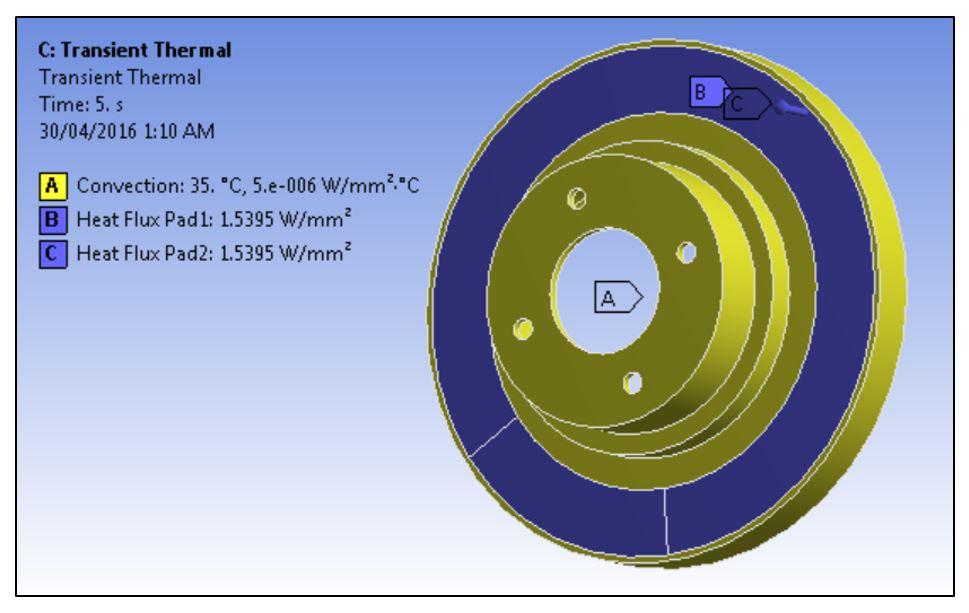
\includegraphics[width=0.6\textwidth]{bc1.jpg}
\caption{Transient thermal boundary conditions}
\label{bc1}
\end{center}
\end{figure}
The temperature plot obtained is as shown in Figure \ref{temp}. As observed, the maximum temperature of $321^{o}C$ is obtained for initial conditions on the design variables.
\begin{figure}[H]
\begin{center}
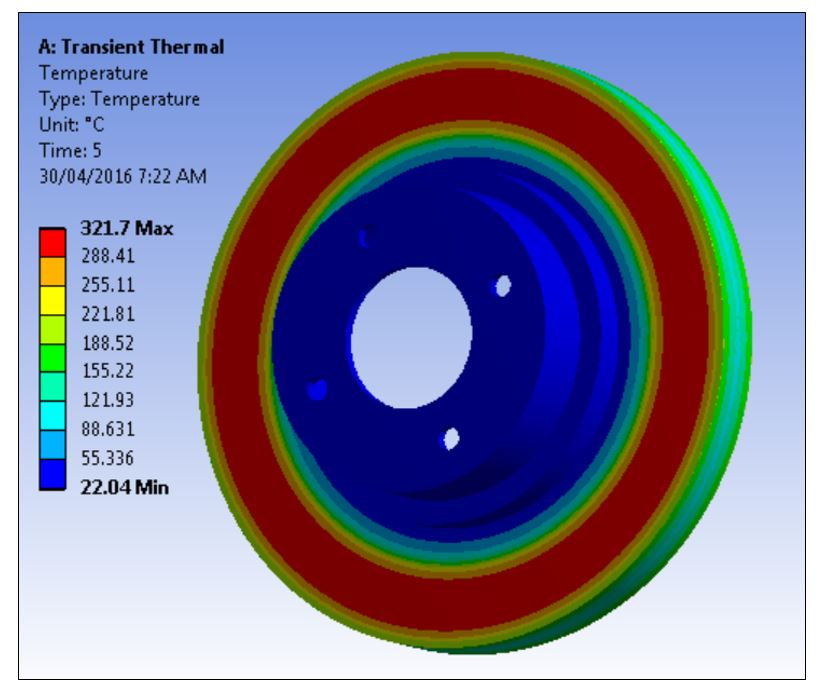
\includegraphics[width=0.55\textwidth]{temp.jpg}
\caption{Temperature plot for initial conditions on the design variables}
\label{temp}
\end{center}
\end{figure}
\subsection{Design of Experiments}
After the initial analysis of each subsystem, the relationship between the design variables and output response is determined. All of the input variables are quantitative and continuous in nature. To obtain the accurate response surface, minimum number of design points from the given sample space are required. Latin Hypercube Sampling (LHS) technique with user defined sample points is used to create the response surface. The main advantage of LHS is that all the sample points are varying in nature. Unlike other sampling methods like Central Composite Design (CCD) and the full factorial methods, the number of simulations required for LHS remains constant even with an increasing number of parameters. After the design of experiments process, we obtain various combinations of input parameters and the corresponding response values. All the 50 DOE points are shown in Appendix A.
\subsection{Response Surface}
After DOE, a response surface is generated for all the input and output values using the least squares methodology. The data points are fitted with a standard $2^{nd}$ order model. The points generated on the response surface are then used to perform the optimization. The goodness of fit plots for all the subsystems are shown below.
\begin{figure}[H]
\begin{center}
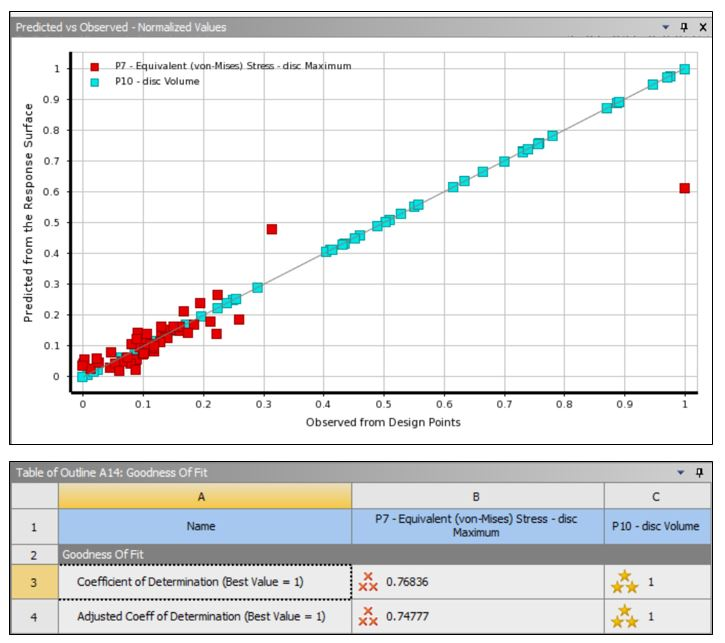
\includegraphics[width=0.75\textwidth]{reg1.jpg}
\caption{Goodness of fit plot for structural analysis}
\end{center}
\end{figure}
\begin{figure}[H]
\begin{center}
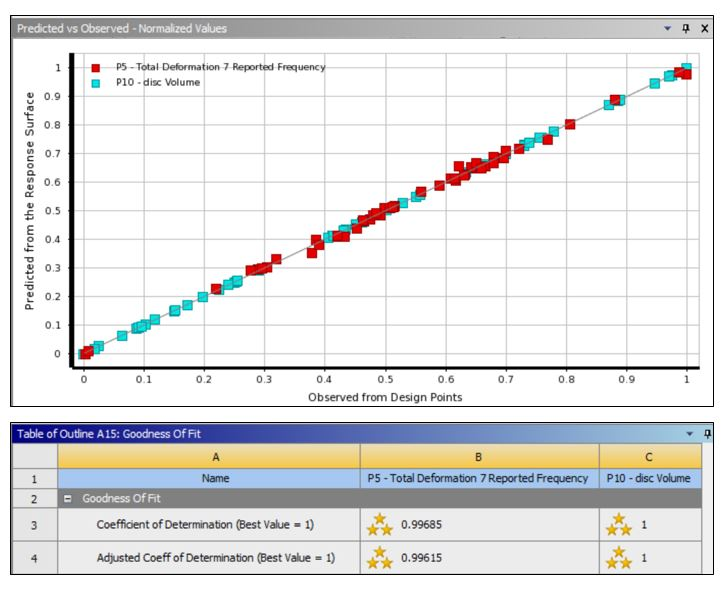
\includegraphics[width=0.65\textwidth]{reg2.jpg}
\caption{Goodness of fit plot for modal analysis}
\end{center}
\end{figure}
\begin{figure}[H]
\begin{center}
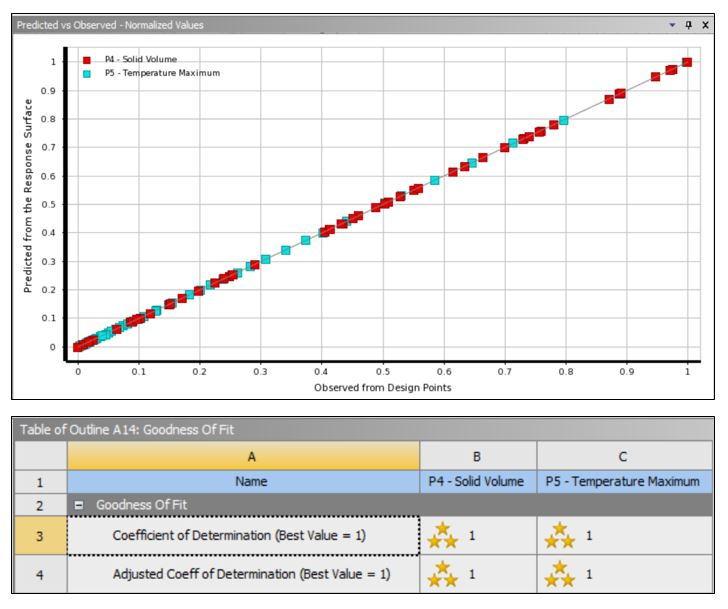
\includegraphics[width=0.65\textwidth]{reg3.jpg}
\caption{Goodness of fit plot for thermal analysis}
\end{center}
\end{figure}
\section{Optimization Study}

\subsection{Structural Analysis Optimization}
For the subsystem 1 optimization problem, the upper bound on the stress constraint from Equation \ref{7} is parametrized and the corresponding optimal volume is evaluated using the \emph{Interior-Point Method (IPM)} in MATLAB. A Pareto curve of optimal volume against the respective stress upper bound is plotted using the IPM and MOGA algorithms as shown in Figure \ref{fig2}. All the MATLAB codes are attached in Appendix B. As observed from the figure, the curves obtained using both the algorithms are in good agreement with each other. Using the Pareto curve, one can easily obtain the optimal volume value for a given stress upper bound constraint. 
\begin{figure}[H]
\begin{center}
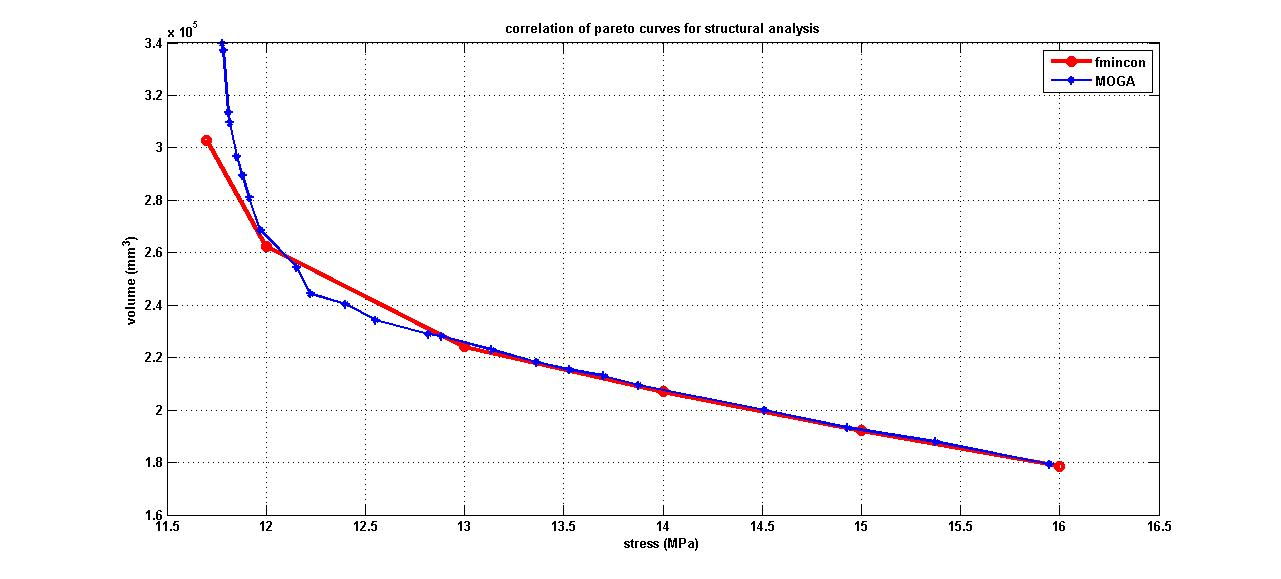
\includegraphics[width=0.9\textwidth]{structural_pareto.jpg}
\caption{Correlation of Pareto curves from IPM (fmincon) and MOGA for structural analysis}
\label{fig2}
\end{center}
\end{figure}
It is observed from the Lagrange multiplier values that constraints $g3, g5$ and $g7$ become active. The design variables optimal values obtained for 14 MPa stress upper bound are correlated with those obtained from ANSYS in the results section. The optimal design variables candidate points obtained in ANSYS by the implementation of MOGA are shown in Figure \ref{cs}. The highlighted candidate point (least volume) is chosen as the best point which is used for validation purposes.
\begin{figure}
\begin{center}
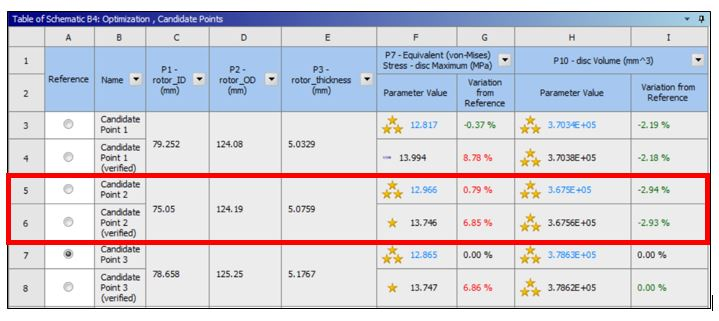
\includegraphics[width=0.9\textwidth]{cs.jpg}
\caption{Optimal dimensions candidate points for structural analysis}
\label{cs}
\end{center}
\end{figure}
\subsection{Modal Analysis Optimization}
For the subsystem 2 optimization problem, the lower bound on the first natural frequency constraint from Equation \ref{8} is parametrized and the corresponding optimal volume is evaluated using IPM in MATLAB. A Pareto curve of optimal volume against the respective frequency lower bound is plotted using the IPM and MOGA algorithms as shown in Figure \ref{fig3}. As observed from the figure, the curves obtained using both the algorithms are in good agreement with each other. Using the Pareto curve, one can easily obtain the optimal volume value for a given frequency lower bound constraint. 
\begin{figure}[H]
\begin{center}
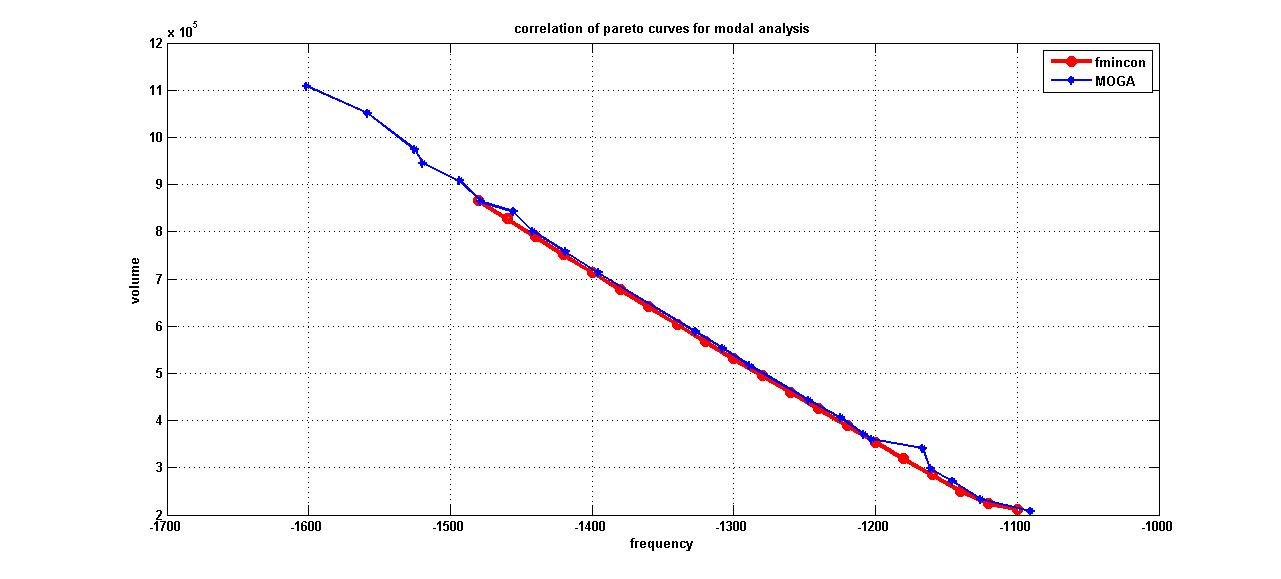
\includegraphics[width=0.9\textwidth]{modal_pareto.jpg}
\caption{Correlation of Pareto curves from IPM (fmincon) and MOGA for modal analysis}
\label{fig3}
\end{center}
\end{figure}
It is observed from the Lagrange multiplier values that constraints $g3$ and $g8$ become active. The design variables optimal values obtained for 1200 Hz frequency lower bound are correlated with those obtained from ANSYS in the results section. The optimal design variables candidate points obtained in ANSYS by the implementation of MOGA are shown in Figure \ref{cn}. The highlighted candidate point (least volume) is chosen as the best point which is used for validation purposes.
\begin{figure}[H]
\begin{center}
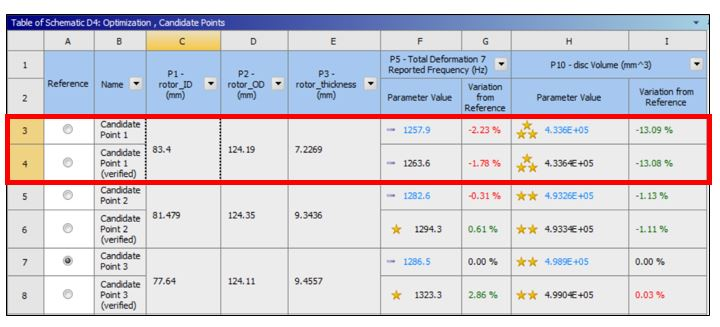
\includegraphics[width=0.9\textwidth]{cn.jpg}
\caption{Optimal dimensions candidate points for modal analysis}
\label{cn}
\end{center}
\end{figure}

\subsection{Thermal Analysis Optimization}
For the subsystem 3 optimization problem, the upper bound on the temperature constraint from Equation \ref{9} is parametrized and the corresponding optimal volume is evaluated using the \emph{Interior-Point Method (IPM)} in MATLAB. A Pareto curve of optimal volume against the respective temperature upper bound is plotted using the IPM and MOGA algorithms as shown in Figure \ref{fig4}. As observed from the figure, the curves obtained using both the algorithms are in good agreement with each other. Using the Pareto curve, one can easily obtain the optimal volume value for a given temperature upper bound constraint. 
\begin{figure}[H]
\begin{center}
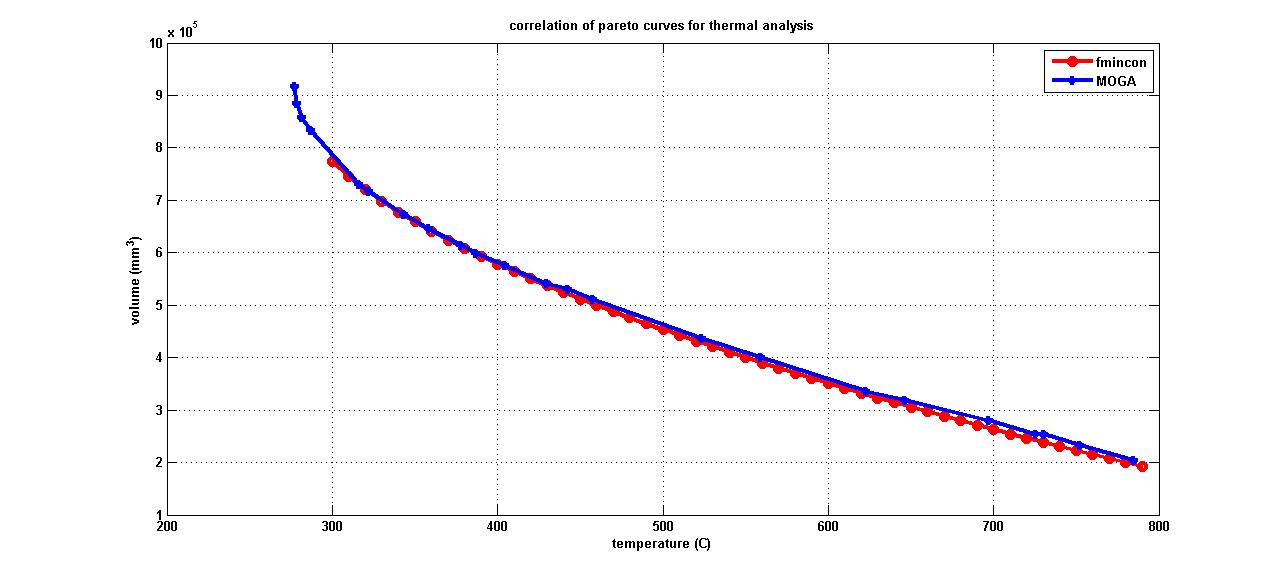
\includegraphics[width=0.9\textwidth]{thermal_pareto.jpg}
\caption{Correlation of Pareto curves from IPM (fmincon) and MOGA for thermal analysis}
\label{fig4}
\end{center}
\end{figure}
It is observed from the Lagrange multiplier values that constraints $g3$ and $g9$ become active. The design variables optimal values obtained for $400^{o}C$ temperature upper bound are correlated with those obtained from ANSYS in the results section. The optimal design variables candidate points obtained in ANSYS by the implementation of MOGA are shown in Figure \ref{ct}. The highlighted candidate point (least volume) is chosen as the best point which is used for validation purposes.
\begin{figure}[H]
\begin{center}
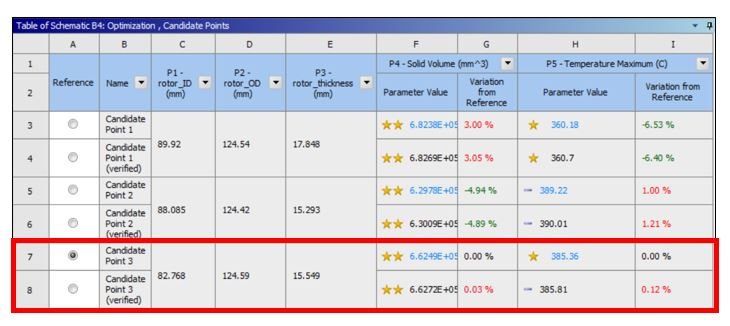
\includegraphics[width=0.9\textwidth]{ct.jpg}
\caption{Optimal dimensions candidate points for thermal analysis}
\label{ct}
\end{center}
\end{figure}
\section{Discussion of Results}
\subsection{Structural Analysis Results}
As observed from the Pareto curves in Figure \ref{fig2}, the optimal volume magnitude increases as the stress upper bound decreases. The objective here is to minimize the stress and volume which ensures a trade-off between the two. This trade-off makes the stress constraint ($g7$) active. The lower bound of the outer radius ($g3$) and thickness ($g5$) constraints are also active. This is confirmed by obtaining and analyzing the Langrange multipliers for all the constraints. Optimal values of the design variables for 14 MPa stress constraint are obtained from MATLAB (fmincon algorithm) and ANSYS (MOGA). Their correlation is shown in Table \ref{corr1}.

\begin{longtable}{|l|c|c|c|c|}
\hline 
\textbf{Parameter} & \textbf{Initial} & \textbf{Optimal value} & \textbf{Optimal value} & \textbf{Error (\%)} \\
 & \textbf{value} & \textbf{from MATLAB (m)} & \textbf{from ANSYS (a)} & \textbf{$(a-m)/m$}\\
\hline
P1 & 75.00 & 78.42 & 75.05 & 1.05 \\
\hline
P2 & 125.00 & 124.00 & 124.19 & 0.15 \\
\hline
P3 & 25.00 & 5.00 & 5.08 & 1.06\\
\hline
S & 14.26 & 14.00 & 13.99 & -0.07 \\
\hline
\caption{Correlation between MATLAB (IPM) and ANSYS (MOGA) optimal values for 14 MPa stress constraint}
\label{corr1}
\end{longtable}
The error values in the table show that the MATLAB and ANSYS optimal values are in good agreement with each other. The stress constraint being active, the optimal stress value obtained from ANSYS should be 14 MPa. But as observed from the Table, the ANSYS value is 14.26 MPa. This has introduced errors in the disc dimension values. These errors will reduce if MOGA generates an optimal stress value closer to 14 MPa in ANSYS.

\subsection{Modal Analysis Results}
As observed from the Pareto curves in Figure \ref{fig3}, the optimal volume magnitude increases as the frequency lower bound increases. The objective here is to maximize the frequency and minimize the volume which ensures a trade-off between the two. This trade-off makes the frequency constraint ($g8$) active. The lower bound of the outer radius ($g3$) constraint is also active. This is confirmed by obtaining and analyzing the Langrange multipliers for all the constraints. Optimal values of the design variables for 1200 Hz frequency constraint are obtained from MATLAB (fmincon algorithm) and ANSYS (MOGA). Their correlation is shown in Table \ref{corr2}.

\begin{longtable}{|l|c|c|c|c|}
\hline 
\textbf{Parameter} & \textbf{Initial} & \textbf{Optimal value} & \textbf{Optimal value} & \textbf{Error (\%)} \\
 & \textbf{value} & \textbf{from MATLAB (m)} & \textbf{from ANSYS (a)} & \textbf{$(a-m)/m$}\\
\hline
P1 & 75.00 & 78.25 & 83.40 & 6.58 \\
\hline
P2 & 125.00 & 124.00 & 124.19 & 0.15 \\
\hline
P3 & 25.00 & 7.76 & 7.23 & -6.82\\
\hline
F & 1590.00 & 1200.00 & 1263.62 & 5.30 \\
\hline
\caption{Correlation between MATLAB (IPM) and ANSYS (MOGA) optimal values for 1200 Hz frequency constraint}
\label{corr2}
\end{longtable}
The error values in the table show that the MATLAB and ANSYS optimal values are in good agreement with each other. The frequency constraint being active, the optimal frequency value obtained from ANSYS should be 1200 Hz. But as observed from the Table, the ANSYS value is 1263.62 Hz. This has introduced errors in the disc dimension values. These errors will reduce if MOGA generates an optimal frequency value close to 1200 Hz in ANSYS.

\subsection{Thermal Analysis Results}
As observed from the Pareto curves in Figure \ref{fig4}, the optimal volume magnitude increases as the temperature upper bound decreases. The objective here is to minimize the temperature and volume which ensures a trade-off between the two. This trade-off makes the temperature constraint ($g9$) active. The lower bound of the outer radius ($g3$) constraint is also active. This is confirmed by obtaining and analyzing the Langrange multipliers for all the constraints. Optimal values of the design variables for $400^{o}C$ temperature constraint are obtained from MATLAB (fmincon algorithm) and ANSYS (MOGA). Their correlation is shown in Table \ref{corr3}.
\newpage
\begin{longtable}{|l|c|c|c|c|}
\hline 
\textbf{Parameter} & \textbf{Initial} & \textbf{Optimal value} & \textbf{Optimal value} & \textbf{Error (\%)} \\
 & \textbf{value} & \textbf{from MATLAB (m)} & \textbf{from ANSYS (a)} & \textbf{$(a-m)/m$}\\
\hline
P1 & 75.00 & 83.16 & 82.77 & -0.46 \\
\hline
P2 & 125.00 & 124.00 & 124.59 & 0.47 \\
\hline
P3 & 25.00 & 13.69 & 15.54 & 13.51\\
\hline
T & 321.70 & 400.00 & 385.81 & -3.54 \\
\hline
\caption{Correlation between MATLAB (IPM) and ANSYS (MOGA) optimal values for $400^{o}C$ temperature constraint}
\label{corr3}
\end{longtable}
The error values in the table show that the MATLAB and ANSYS optimal values are in good agreement with each other. The temperature constraint being active, the optimal temperature value obtained from ANSYS should be $400^{o}C$. But as observed from the Table, the ANSYS value is $321.7^{o}C$. This has introduced errors in the disc dimension values. These errors will reduce if MOGA generates an optimal stress value closer to $400^{o}C$ in ANSYS.

\section{System Integration Study}
After performing the individual subsystem level optimization, an attempt is made to integrate all the subsystems. There are four objective functions in this problem. As it is not possible to plot 4D Pareto curves, three objective functions are considered at a time so that 3D Pareto curves can be easily plotted from them in MATLAB. This study helps us understand the relationship between three objective functions at a time.
\subsection{Combined Modal \& Thermal Optimization}
The mathematical model for this system level optimization is as follows:\newline\newline
$Min: f1, -f3, f4$\\\\
s.t.\\  $g1, g2, g3, g4, g5, g6, g8$ and $g9$\\\\
Optimization is performed in MATLAB using the single objective IPM (fmincon) method. This algorithm being used for single objective optimization problem, the volume function is considered to be the primary objective and the frequency and temperature objective functions are considered as constraints. The lower and upper bounds on frequency and temperature respectively are varied and a Pareto curve for volume, frequency and temperature is obtained as shown in Figure \ref{pareto1}. The optimal volume value for 1200 Hz lower bound on frequency and $400^{o}C$ upper bound on temperature is obtained from this Pareto curve and is correlated with a MOGA value obtained from ANSYS.
\begin{figure}[H]
\begin{center}
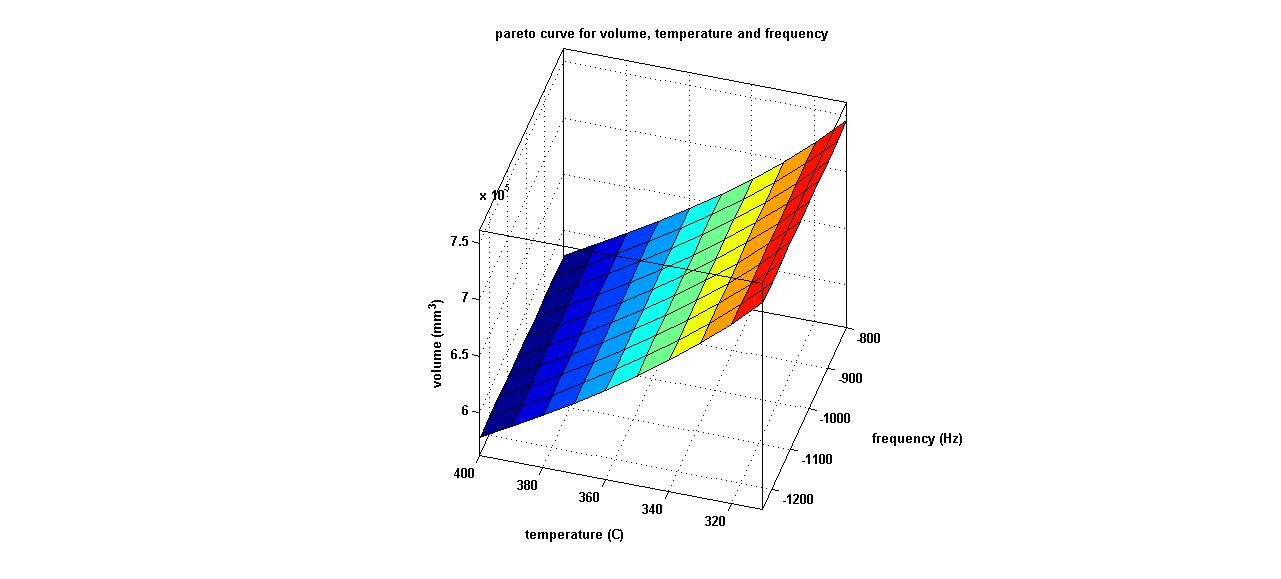
\includegraphics[width=1.1\textwidth]{temp_freq_pareto.jpg}
\caption{Pareto curve for volume, frequency and temperature}
\label{pareto1}
\end{center}
\end{figure}
As observed from this Pareto curve, for a given temperature constraint, the optimal volume does not vary with the frequency constraint. Thus, we have the temperature constraint ($g9$) active. This is verified from the Lagrange multipliers obtained from MATLAB. MATLAB (fmincon algorithm) and ANSYS (MOGA) correlation for one of the temperature and frequency constraints is presented in Table \ref{2con1}. The candidate points obtained from ANSYS are shown in Figure \ref{mt}. The highlighted point (least volume) is chosen as the best optimal point.
\begin{figure}[H]
\begin{center}
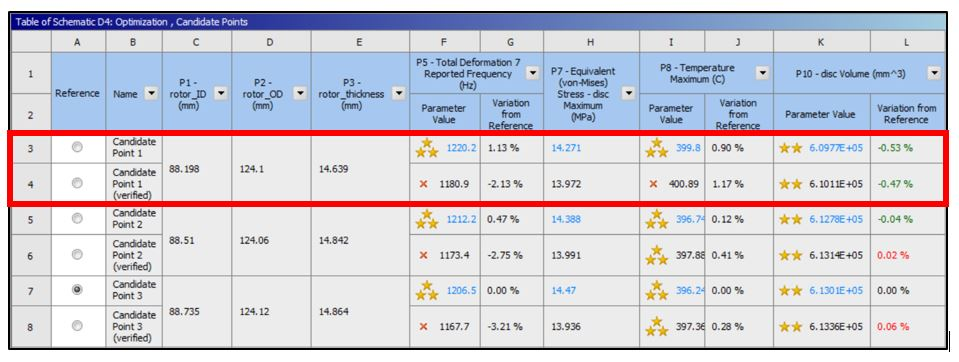
\includegraphics[width=1\textwidth]{mt.jpg}
\caption{Optimal dimensions candidate points for combined modal and thermal analysis}
\label{mt}
\end{center}
\end{figure}
\newpage
\begin{longtable}{|l|c|c|c|c|}
\hline 
\textbf{Parameter} & \textbf{Initial} & \textbf{Optimal value} & \textbf{Optimal value} & \textbf{Error (\%)} \\
 & \textbf{value} & \textbf{from MATLAB (m)} & \textbf{from ANSYS (a)} & \textbf{$(a-m)/m$}\\
\hline
P1 & 75.00 & 83.16 & 88.19 & 6.04 \\
\hline
P2 & 125.00 & 124.00 & 124.10 & 0.08 \\
\hline
P3 & 25.00 & 13.69 & 14.64 & 6.93\\
\hline
F & 1590.00 & 1310.60 & 1220.20 & -6.89 \\
\hline
T & 321.70 & 400.00 & 399.80 & -0.05 \\
\hline
\caption{Correlation between MATLAB and ANSYS optimal values for 1200 Hz frequency constraint and $400^{o}C$ temperature constraint}
\label{2con1}
\end{longtable}
As observed from the Table \ref{2con1}, there is no significant difference in the error percentage between ANSYS and MATLAB values. Moreover, MATLAB gives a better optimal point (lower dimensions and volume) as compared to the ANSYS value. MOGA solutions do not satisfy the KKT conditions. The initial volume being $9.96*10^{5} mm^{3}$, MATLAB optimal solution gives the minimum volume to be $5.78*10^{5} mm^{3}$ i.e. an improvement in the volume reduction of \textbf{41.9\%}.
\subsection{Combined Modal \& Structural Optimization}
The mathematical model for this system level optimization is as follows:\newline\newline
$Min: f1, f2, -f3$\\\\
s.t.\\  $g1, g2, g3, g4, g5, g6, g8$ and $g7$\\\\
Optimization is performed in MATLAB using the single objective IPM (fmincon) method. This algorithm being used for single objective optimization problem, the volume function is considered to be the primary objective and the frequency and stress objective functions are considered as constraints. The lower and upper bounds on frequency and stress respectively are varied and a Pareto curve for volume, frequency and stress is obtained as shown in Figure \ref{pareto2}. The optimal volume value for 1200 Hz lower bound on frequency and 14 MPa upper bound on stress is obtained from this Pareto curve and is correlated with a MOGA value obtained from ANSYS.
\begin{figure}
\begin{center}
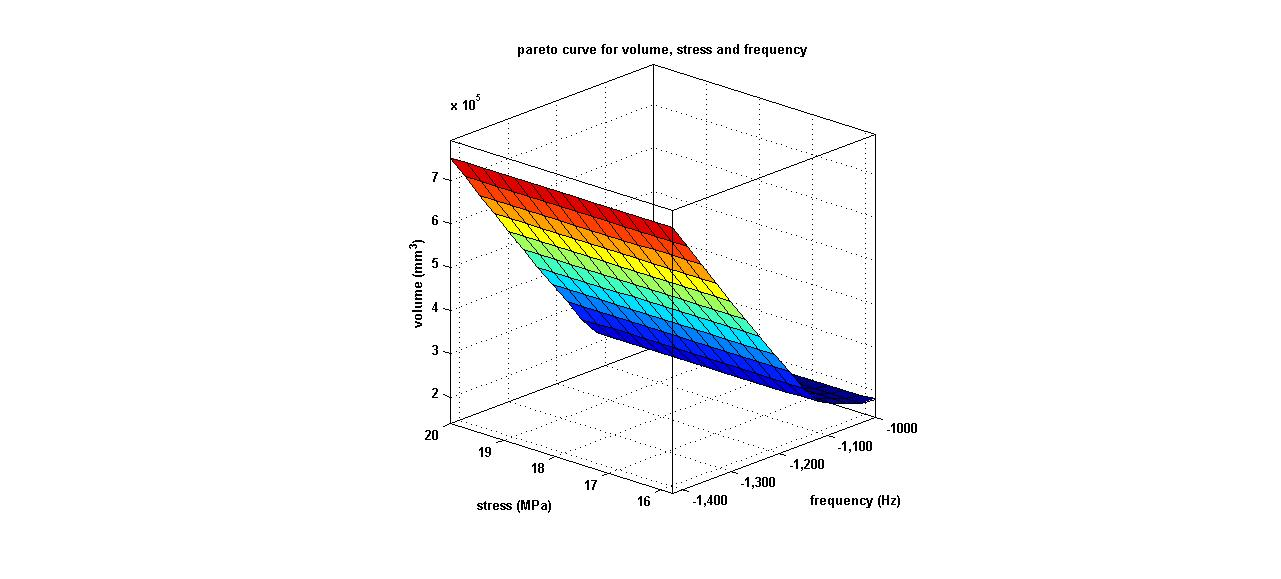
\includegraphics[width=1\textwidth]{stress_freq_pareto.jpg}
\caption{Pareto curve for volume, frequency and stress}
\label{pareto2}
\end{center}
\end{figure}
As observed from this Pareto curve, for a given frequency constraint, the optimal volume doesn't vary with the stress constraint. Thus, we have the frequency constraint ($g8$) active. This is verified from the Lagrange multipliers obtained from MATLAB. MATLAB (fmincon algorithm) and ANSYS (MOGA) correlation for one of the stress and frequency constraints is presented in Table \ref{2con2}. The candidate points obtained from ANSYS are shown in Figure \ref{ms}. The highlighted point (least volume) is chosen as the best optimal point.
\begin{figure}[H]
\begin{center}
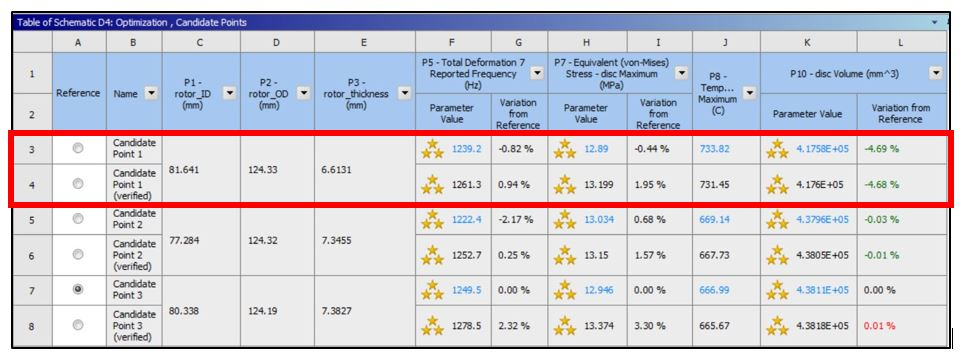
\includegraphics[width=0.9\textwidth]{ms.jpg}
\caption{Optimal dimensions candidate points for combined modal and structural analysis}
\label{ms}
\end{center}
\end{figure}
\begin{longtable}{|l|c|c|c|c|}
\hline 
\textbf{Parameter} & \textbf{Initial} & \textbf{Optimal value} & \textbf{Optimal value} & \textbf{Error (\%)} \\
 & \textbf{value} & \textbf{from MATLAB (m)} & \textbf{from ANSYS (a)} & \textbf{$(a-m)/m$}\\
\hline
P1 & 75.00 & 78.25 & 81.64 & 4.33 \\
\hline
P2 & 125.00 & 124.00 & 124.33 & 0.26 \\
\hline
P3 & 25.00 & 7.76 & 6.61 & -14.81\\
\hline
F & 1590.00 & 1200 & 1261.30 & 5.10 \\
\hline
S & 14.26  & 12.77 & 13.20 & 3.36 \\
\hline
\caption{Correlation between MATLAB and ANSYS optimal values for 1200 Hz frequency constraint and 14 MPa stress constraint}
\label{2con2}
\end{longtable}
\newpage
As observed from the Table \ref{2con2}, there is no significant difference in the error percentage between ANSYS and MATLAB values. Moreover, MATLAB gives a better optimal point (lower dimensions and volume) as compared to the ANSYS value. The initial volume being $9.96*10^{5} mm^{3}$, MATLAB optimal solution gives the minimum volume of $3.54*10^{5} mm^{3}$ i.e. an improvement in the volume reduction of \textbf{64.4\%}.
 \subsection{Combined Structural, Modal \& Thermal Optimization}
The mathematical model for this system optimization is as follows:\newline\newline
$Min: f1, f2, -f3,f4$\\\\
s.t.\\  $g1, g2, g3, g4, g5, g6$ \\\\
This combined system level optimization is performed in MATLAB and ANSYS using the MOGA algorithm. The optimization procedure is as shown in Figure \ref{doe_all}. 
\begin{figure}[H]
\begin{center}
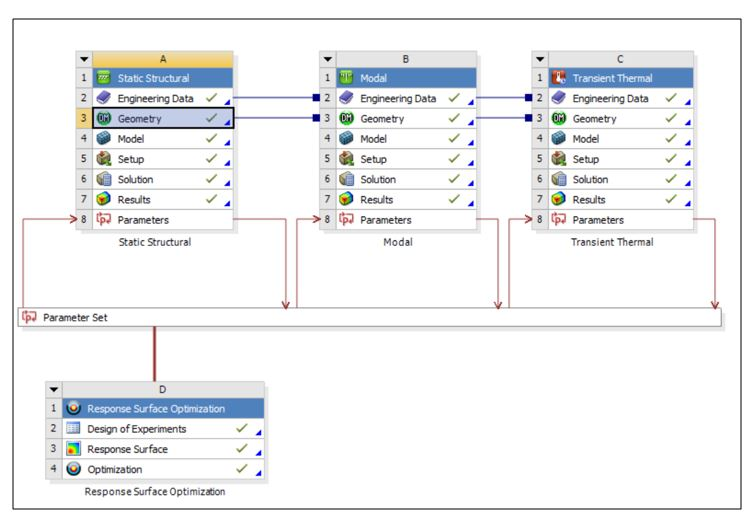
\includegraphics[width=1\textwidth]{doe_all.jpg}
\caption{System optimization procedure}
\label{doe_all}
\end{center}
\end{figure}
Corresponding points chosen from MATLAB and ANSYS are validated in Table \ref{2con3}. The highlighted point (least volume) from Figure \ref{global} is chosen as the best optimal point.
\begin{figure}[H]
\begin{center}
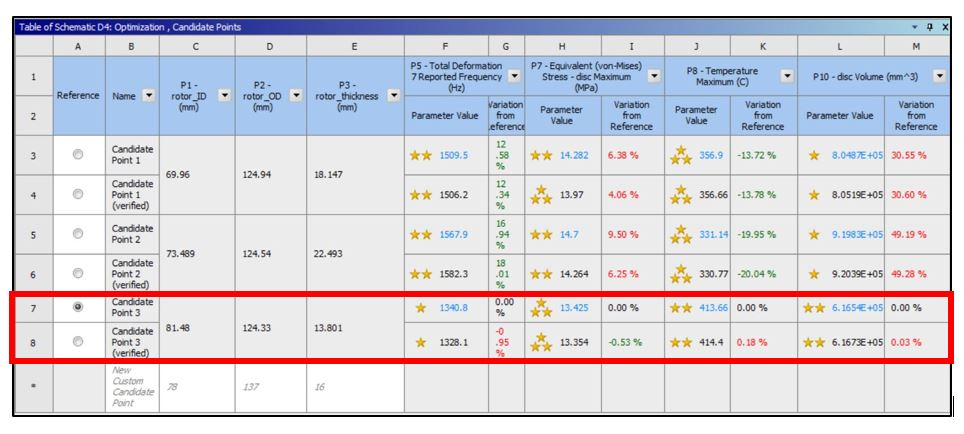
\includegraphics[width=0.9\textwidth]{mg.jpg}
\caption{Optimal dimensions candidate points for combined structural, modal and thermal analysis}
\label{global}
\end{center}
\end{figure}
\begin{longtable}{|l|c|c|c|c|}
\hline 
\textbf{Parameter} & \textbf{Initial} & \textbf{Optimal value} & \textbf{Optimal value} & \textbf{Error (\%)} \\
 & \textbf{value} & \textbf{from MATLAB (m)} & \textbf{from ANSYS (a)} & \textbf{$(a-m)/m$}\\
\hline
P1 & 75.00 & 76.11 & 81.48 & 7.05 \\
\hline
P2 & 125.00 & 124.83 & 124.33 & -0.40 \\
\hline
P3 & 25.00 & 14.34 & 13.80 & -3.76\\
\hline
F & 1590.00 & 1340.60 & 1328.1 & -0.93 \\
\hline
S & 14.26  & 13.28 & 13.35 & 0.53 \\
\hline
T & 321.70  & 370.75 & 414.40 & 11.77 \\
\hline
V & 9.96*$10^{5}$ & 6.45*$10^{5}$ & 6.17*$10^{5}$ & -4.34 \\
\hline
\caption{Correlation between MATLAB and ANSYS optimal values for combined structural, modal and thermal analysis using MOGA}
\label{2con3}
\end{longtable}
As observed from Table \ref{2con3}, the initial volume being 9.96*$10^{5} mm^{3}$, MATLAB optimal solution gives the minimum volume as 6.45*$10^{5} mm^{3}$ i.e. an improvement in the volume reduction of \textbf{35.2\%}. The final optimal dimensions (P1, P2 and P3) as given by the MOGA algorithm in MATLAB are 76.11 mm, 124.83 mm and 14.34 mm respectively.
\begin{figure}[H]
\begin{center}
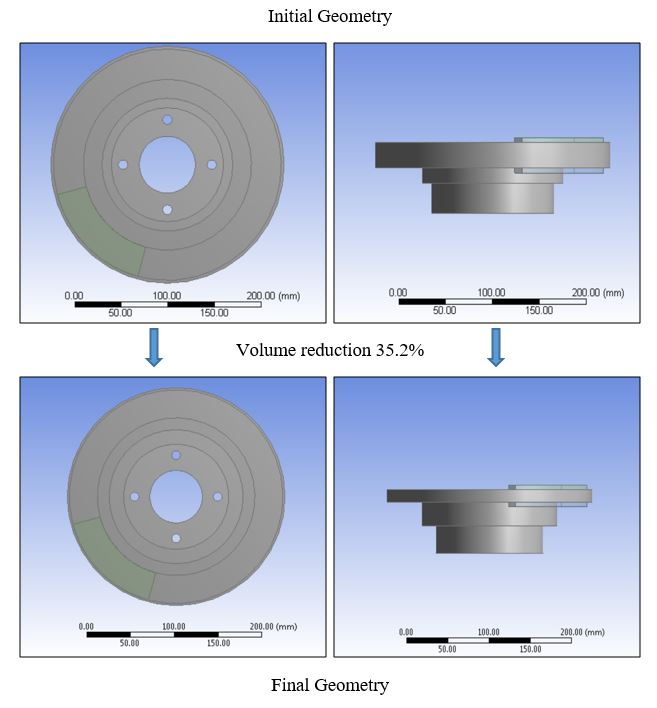
\includegraphics[width=0.8\textwidth]{geom.jpg}
\caption{Initial and final brake disc geometries}
\label{geom}
\end{center}
\end{figure}
\section{References}
[1] 	P. Y. Papalambros, Principles of Optimal Design: Modeling and Computation, 2016. \newline\newline
[2] 	M. Reibenschuh et. al, Modelling and Analysis of Thermal and Stress Loads in Train Disc Brakes – Braking from 250 km/h to Standstill, \emph{Journal of Mechanical Engineering}, 2009. \newline\newline
[3] 	D. C. Montgomery, Design and Analysis of Experiments, John Wiley \& Sons, Inc., Eighth Edition. \newline\newline
[4] 	G. M. Nathy et. al, Coupled Structural / Thermal Analysis of Disc Brake, \emph{IJRET}. \newline\newline
[5] 	ANSYS and MATLAB manual. \newline\newline
[6] 	M. Reibenschuh and F. Cus, Stress Analysis Of A Brake Disc Considering Centrifugal Load, \emph{Journal of Production Engineering}, Vol. 12. \newline\newline
[7] 	Y. Ren, MAE 598 - Design Optimization Notes, 2016.
\newpage
\section{Appendix}
\subsection A
The DOE points obtained using the LHS method are as follows:
\begin{figure}[H]
\begin{center}
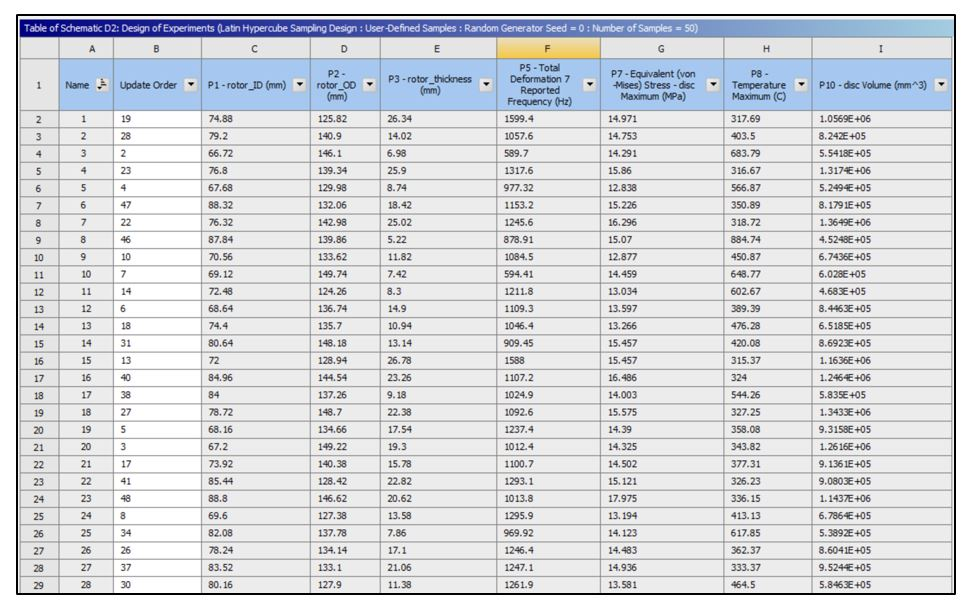
\includegraphics[width=0.65\textwidth]{doe1.jpg}
\caption{LHS DOE points}
\end{center}
\end{figure}
\begin{figure}[H]
\begin{center}
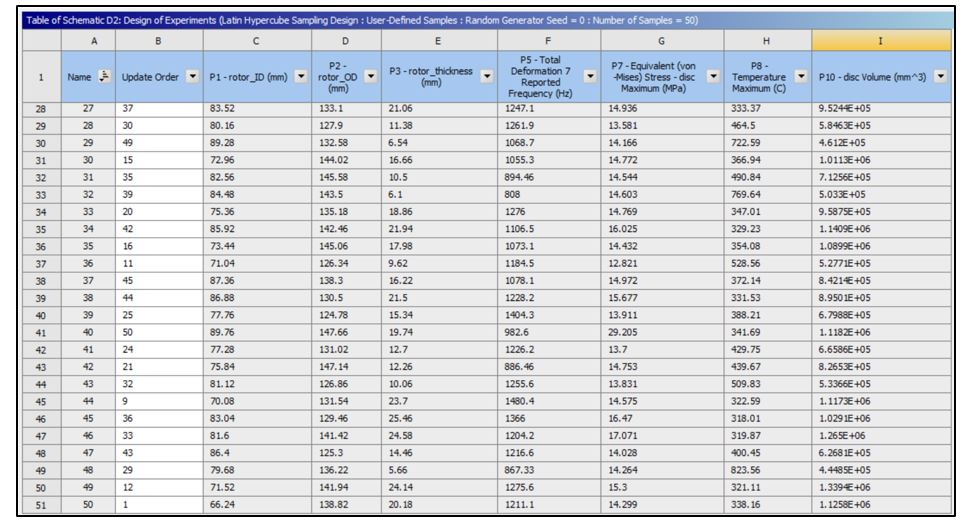
\includegraphics[width=0.65\textwidth]{doe2.jpg}
\caption{LHS DOE points (continued)}
\end{center}
\end{figure}
\subsection B
MOGA and fmincon (IPM) MATLAB codes for subsystem and combined system level optimization are attached below. Respective excel sheet containing all the DOE points should be provided for the codes to work. The subsystem level codes provided are only for the modal analysis. Changes can be easily made to make them work for structural and thermal analyses.
%\\Motivation\\Nomenclature\\Introduction\\Flowchart\\CAD Model\\FEM Analysis\\DOE\\Metamodelling\\MATLAB Optimization\\ANSYS Optimization\\Result Validation\\Conclusion\\References\\Appendix (codes)
\end{document}
